\documentclass[11pt]{article}

%
% Template for GFD reports.
%
% Updated 12/2000.  Address all complaints to Jean-Luc Thiffeault,
% jeanluc@mailaps.org
%
% Updated for 2004 (SDM).
%

%
% Packages (do not delete any!)
%

% This package handles embedded postscript figures.
\usepackage{graphicx}
% The amsmath and amssymb packages provide some extra commands/fonts.
\usepackage{amsmath,amssymb}

% The margins:
\usepackage[body={6in,8.5in}]{geometry}

% LEAVE THESE NEXT TWO LINES IN (used in final version for page numbering).
%\usepackage{lastpage,xr}
%\externaldocument[pr-]{../<previousrep>/rep_<previousrep>}

% The citation format to use.
\bibliographystyle{pfa}

% Add your own packages here, if necessary.

%
% Definitions
%
%
% Symbols file GFD2002
%

% Partial derivative
\def\pd{\partial}
% Real numbers
\def\reals{{\mathbb R}}
% 1st partial derivative
\newcommand {\pdd}[2]{\frac{\partial #1}{\partial #2}}
% 2nd partial derivative
\newcommand {\pdTwo}[2]{\frac{\partial^{2} #1}{\partial #2^{2}}}
% reference style
%\newcommand {\nref}[1]{~(\ref{#1})}
\newcommand {\nref}[1]{~\ref{#1}}
% unit vector notation
\newcommand {\unitv}[1]{\mathbf{\hat{#1}}}
% the subscript for the horizontal component
\newcommand {\horiz}{_{_{H}}}
% the symbol for the velocity
\newcommand {\vel}{\mathbf{u}}
% the symbol for the horizontal velocity
\newcommand {\uh}{\vel\horiz}
% the symbol for the vertical unit vector
\newcommand {\khat}{\unitv{k}}
% the symbol for the unit vector in th y direction
\newcommand {\jhat}{\unitv{j}}
% the symbol for the unit vector in the direction \hnabla h
\newcommand {\nhat}{\unitv{n}}
% the symbol for the horizontal nabla
\newcommand {\hnabla}{\nabla\!\horiz}
% the symbol for the horizontal laplacian
\newcommand {\hlap}{\hnabla^{\,2}}
% the subscript denoting top
\newcommand {\up}{_{_{T}}}
% the subscript denoting bottom
\newcommand {\down}{_{_{B}}}
% degree symbol
\newcommand {\degree} {^{\circ}}
% Cross product
\def\cross{\times}


% Define your own commands here, or input them externally (say, mysymbols.tex).
%\input{mysymbols}

%
% Title
%
\title{The Role of Tidal Dissipation \\ and the Laplace Tidal Equations}
\author{Myrl Hendershott}

\begin{document}

\maketitle

% LEAVE THESE NEXT TWO LINES IN (used in final version for page numbering).
% They must go right after the \maketitle command.
%\setcounter{page}{\pageref{pr-LastPage}}
%\addtocounter{page}{1}

\section{Introduction}
\label{Intro}

In this lecture we make a first attempt to describe the dynamics of tides. We first provide some discussion of their influence on the global processes of the earth by relating tidally induced dissipation to the change in the earth's rotation rate, and consider whether there is any fossil evidence of such a change. We then approach this question of dissipation a little more formally, from the perspective of an angular momentum budget of the earth-moon system. Finally, we develop the dynamics of tides from first principles, starting with the Navier-Stokes equations on a rotating planet and, after imposing a Boussinesq approximation and decomposing the linearized equations into vertical modes, deriving the Laplace tidal equations.

%%%%%%%%%%%%%%%%%%%%%%%%%%%%%%%%%%%%%%%%%%%%%%%%%%%%%%%%%%%%%%%%%%%%%%%%%%%%%%%

\section{Energetic Dissipation}
\label{EnergyDissipation}

% Neil says that the logic of this section is backwards. I suppose that he's right... but shit, this is Myrl's presentation!! What am I supposed to do about this?

We shall first consider the relationship between tidal dissipation and the rotation rate of the earth. If we neglect the internal dynamics of the earth, regarding it as a collection of processes that will eventually lead to dissipation, then the persistent energy of the planet is due to rigid-body rotation, whose rate of change is
\begin{equation}
E_t = \pdd{}{t} \left(\tfrac{1}{2} C \Omega^2 \right),
\end{equation}
where $C$ is the earth's moment of inertia along the polar axis and $\Omega$ is the earth's rotation rate. The change in $\Omega$ is then given by
\begin{equation}
\label{EarthRotationRate}
\Omega_t = \frac{E_t}{C \Omega}.
\end{equation}

In most circumstances, astronomical data is used to infer $\Omega_t$, which is then used to compute $E_t$. But to help motivate this relationship, we would like to compare it to some sort of observational record. For the moment, let us suppose that we have some rough estimate for the tidal dissipation. We may then use this to demonstrate how this lead to a variation in the length of day. Such variation could then leave an imprint in the fossil records, for example. So in this case, if we use the following values,\cite{Lambeck}
\begin{align*}
E_t &= -4.0 \times 10^{19} \ \textrm{erg} \ \textrm{sec}^{-1}, \\
C &= 8.043 \times 10^{44} \ \textrm{g} \ \textrm{cm}^2, \\
\Omega &= \frac{2 \pi}{86164 \ \textrm{sec}} = 7.292 \times 10^{-5} \ \textrm{sec}^{-1}, \\
\end{align*}
then we would presume that the earth's rotation rate is currently decreasing at about
\begin{equation*}
\Omega_t = - 6.8 \times 10^{-22} \ \textrm{rad} \ \textrm{sec}^{-2}.
\end{equation*}
We can use this to estimate the variation in length of day (LOD),\footnote{The angular rotation per day is slightly greater than $2\pi$, but the error is insignificant for our purposes.}
\begin{equation*}
\begin{split}
\Delta(\textrm{LOD}) &= \tau' - \tau \\
&= 2 \pi \left(\frac{1}{\Omega'} - \frac{1}{\Omega} \right), \\
\end{split}
\end{equation*}
where
\begin{equation*}
\Omega' = \Omega + \Delta\Omega \simeq \Omega + \Omega_t \Delta t,
\end{equation*}
so that
\begin{equation}
\begin{split}
\Delta(\textrm{LOD}) &\simeq -\left(\frac{2 \pi}{\Omega}\right) \left(\frac{\Omega_t}{\Omega}\right) \Delta t  \\
 &= 6.9 \times 10^{-8} \ \textrm{sec}
\end{split}
\end{equation}
for $\Delta t = \textrm{1 day} = 86400 \ \textrm{sec}$. Or, in more appropriate units,
\begin{equation*}
\Delta(\textrm{LOD}) / \textrm{day} = 2.5 \ \textrm{msec} \ \textrm{cy}^{-1}.
\end{equation*}

As long as $\Omega_t \Delta t \ll \Omega$ remains a reasonably accurate statement, it should be possible to extrapolate about the LOD over epochal times. If we take $-\Delta t$ to be 400 million years, then $\Omega_t \Delta t \approx 0.12 \Omega$ and our estimate for a constant LOD variation should be accurate within about $10\%$. Then in we compare the difference between current years and 400 million years ago, we find the following:
\begin{center}
\begin{tabular}{|c|c|}
\hline
        Today         & 365 days per year \\
\hline
400 Million Years Ago & 414 days per year \\
\hline
\end{tabular}
\end{center}
Although the accuracy is a somewhat questionable, it does demonstrate that there has likely been a significant change in both the dynamical and radiation cycle of the earth. A natural question is whether there is any evidence supporting the conjecture that the LOD was longer in the past, and how much $\Omega_t$ and $E_t$ may have varied. The fossil record offers a strong possibility, since biological activity should be sensitive to variations in the radiation cycle; this is explored in the next section.

%%%%%%%%%%%%%%%%%%%%%%%%%%%%%%%%%%%%%%%%%%%%%%%%%%%%%%%%%%%%%%%%%%%%%%%%%%%%%%%

\section{Biological Records}
\label{BioRecords}

% ...Get some pictures here. Find a scanner.

Several groups of organisms leave records in the skeletal parts of their accreting tissue, in the form of sequential and repetitive layers. These layers are interpreted in growth increments, and the sequence of layers appears to be a consequence of modulation of growth by internal rhythms inherent to the animal and environmental conditions.

Growth patterns that are controlled by astronomical phenomena are of particular interest. A comparison of frequencies found in living and fossil specimens may reveal indications of the constancy or periodicity of certain astronomical phenomena. One of the types of organisms that have been studied in a geophysical context is corals.

Seasonal fluctuations in the rate of coral growth were first reported by R. P. Whitefield in 1898, who described undulations on some surfaces of living corals and suggested that these represented annual growth increments associated with seasonal water temperature changes. However, the detailed mechanism by which growth occurs and the factors controlling the rate of growth are still inadequately understood.

The skeletal part of corals consist of several elements, one of which, the epitheca, reveals a fine structure of ridges that are parallel to the growing edge (figure 1). These ridges are interpreted as growth increments and they suggest a periodic fluctuation in the rate of calcium carbonate secretion. The rate of deposition of these growth increments in modern reef-forming corals is believed to be daily.

An indication that the growth ridges are daily is that modern corals typically add about 360 such increments per year, suggesting that the solar day controls the frequency of deposition\cite{Wells1963,Barnes1972}. Although, factors other than variable daylight may be important here in modulating the growth rates, indirect evidence suggests that the solar day has remained the dominant periodicity in corals studied; Devonian corals studied by Wells\cite{Wells1963} show about 400 daily growth increments between successive seasonal annulations, in keeping with expected value, if present tidal acceleration of the Earth has remained roughly constant over last $3\textrm{--}4 \times 10^8$ years. The same qualitaive results can be found in molluscs and stromatolites too.
\begin{figure}
\begin{center}
\resizebox{0.8\textwidth}{!}{
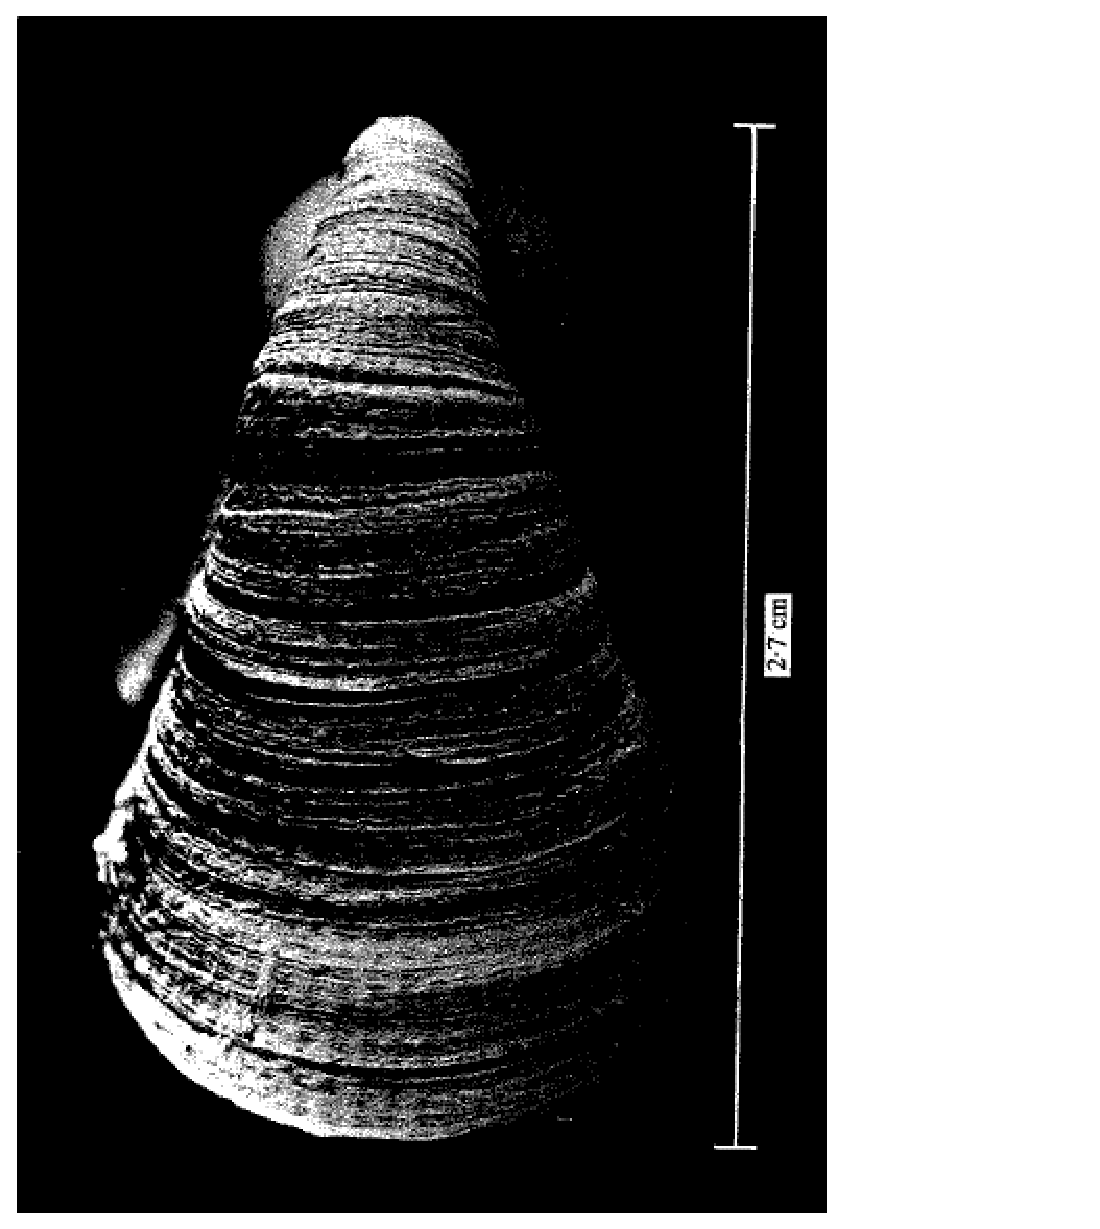
\includegraphics{coral.eps}}
\caption{Middle Devonian coral epitheca from Michigan, U.S.A.}
\label{}
\end{center}
\end{figure}
% ...Add some comment on the other animals.

%%%%%%%%%%%%%%%%%%%%%%%%%%%%%%%%%%%%%%%%%%%%%%%%%%%%%%%%%%%%%%%%%%%%%%%%%%%%%%%

\section{Angular Momentum}
\label{AngMomentum}

% ...Maybe make a stupid moon-around-the-earth picture for this

The consequences of tidal dissipation can also be seen in the receding of the moon from the earth. If we ignore the rotation of the moon and regard it as a point in space moving in a simple circular orbit, and again focus on the rigid-body rotation of the earth, then the total angular momentum of the earth-moon system is conserved and
\begin{equation}
\pdd{}{t} \left(C \Omega + m l^2 \omega \right) = 0,
\end{equation}
where $m$ is the moon's mass, $l$ is the orbital radius, and $\omega$ is the orbital frequency. These parameters currently have values of
\begin{align*}
m &= 7.35 \times 10^{25} \ \textrm{g}, \\
l &= 3.84 \times 10^{10} \ \textrm{cm}, \\
\omega &= \frac{2 \pi}{27.32166 \times 86400 \ \textrm{sec}} = 2.66 \times 10^{-6} \ \textrm{rad} \ \textrm{sec}^{-1}. \\
\end{align*}
Expansion of the angular momentum equation gives
\begin{equation*}
C \Omega_t + m \left(2 l \omega l_t + l^2 \omega_t \right) = 0.
\end{equation*}
To relate the change in distance to the change in frequency, we note that since the motion is circular,
\begin{equation*}
\frac{GMm}{l^2} = m \omega^2 l,
\end{equation*}
so that
\begin{equation*}
\omega^2 l^3 = GM \ \ \ (\textrm{Kepler's Third Law}), % Fix this
\end{equation*}
and hence
\begin{equation}
\label{MoonRotationRate}
\omega_t = -\frac{3}{2} \left(\frac{\omega}{l} \right) l_t.
\end{equation}
We then obtain an expression for the rate at which the moon drifts from the earth,
\begin{equation}
\label{OrbitalRadiusRate}
l_t = -\frac{2 C \Omega_t}{m l \omega}.
\end{equation}
Laser ranging of the moon tells us that
\begin{equation*}
l_t = 3.8 \ \textrm{cm} \ \textrm{yr}^{-1} = 1.2 \times 10^{-7} \ \textrm{cm} \ \textrm{sec}^{-1}
\end{equation*}
from which we infer that the change in the lunar cycle is
\begin{equation*}
\omega_t = -1.25 \times 10^{-23} \ \textrm{rad} \ \textrm{sec}^{-2} = -25.7^{\prime\prime} \ \textrm{cy}^{-2}.
\end{equation*}
This simple estimate is in close agreement with a more sophisticated calculation by Brosche and S\"undermann, who obtained a result of $-26.06^{\prime\prime} \ \textrm{cy}^{-2}$.\cite{Brosche1977}

From equation~\eqref{OrbitalRadiusRate}, we find that the rate of change of the earth's rotation is
\begin{equation*}
\Omega_t = -5.6 \times 10^{-22} \ \textrm{rad} \ \textrm{sec}^{-1}.
\end{equation*}
Based on this rotation rate, the loss of energy of the moon, from equation~\eqref{EarthRotationRate}, is
\begin{equation*}
E_t = -3.3 \times 10^{19} \ \textrm{erg} \ \textrm{sec}^{-1} = -3.3 \ \textrm{TW}
\end{equation*}
which, despite our idealizations, is in good agreement with more sophisticated astronomical calculations of $3.75 \pm 0.08 \ \textrm{TW}$.\cite{Kantha1998}

%%%%%%%%%%%%%%%%%%%%%%%%%%%%%%%%%%%%%%%%%%%%%%%%%%%%%%%%%%%%%%%%%%%%%%%%%%%%%%%

\section{Terrestrial Coordinates and the Traditional Approximation}

There is strong evidence that tides have an impact on the dynamics of the earth, and it therefore seems justifiable to approach them from first principles and develop a consistent set of equations to describe their effects. In this section we consider the dynamics of a shallow fluid on a rotating planet. Later sections will introduce further approximations, which will lead us to the Laplace tidal equations (LTE) for each vertical mode.

The Navier-Stokes equations for an incompressible rotating fluid in spherical (terrestrial) coordinates are
\begin{subequations}
\begin{align}
\frac{D_s u}{Dt} - \left[2\Omega + \frac{u}{r \cos \theta} \right] v \sin \theta + \left[2\Omega + \frac{u}{r \cos \theta} \right] w \cos \theta &= - \frac{p_\phi}{\rho r \cos \theta} - \frac{\Phi_\phi}{r \cos \theta} + X, \\
\frac{D_s v}{Dt} + \left[2\Omega + \frac{u}{r \cos \theta}\right] u \sin \theta + \left[\frac{v}{r}\right] w &= - \frac{p_\theta}{\rho r} - \frac{\Phi_\theta}{r} + Y, \\
\frac{D_s w}{Dt} - \left[\frac{v}{r}\right]v  - \left[2\Omega + \frac{u}{r \cos \theta} \right] u \cos \theta &= - \frac{p_r}{\rho} - \Phi_r + Z, \\
\frac{1}{r \cos \theta} \left[u_\phi + \left(v \cos \theta \right)_\theta \right] + \frac{1}{r^2} \left(r^2 w \right)_r &= 0,
\end{align}
\end{subequations}
where $\theta$ and $\phi$ are the latitude and longitude, $\Phi$ is the geopotential, and $\mathbf{X} = \left(X,Y,Z\right)$ represent dissipative forces. The advective derivative, $\frac{D_s}{Dt}$, is
\begin{equation*}
\frac{D_s}{Dt} = \pdd{}{t} + \frac{u}{r \cos \theta} \pdd{}{\phi} + \frac{v}{r} \pdd{}{\theta} + w \pdd{}{r}
\end{equation*}
and the self-gravitating potential of the earth, including centrifugal forcing, is
\begin{equation}
\Phi = - \frac{G M_E}{r} + A(r, \theta) - \frac{1}{2} \Omega^2 r^2 \cos^2 \theta,
\end{equation}
where $A(r, \theta)$ describes the deviation of gravitation from a spherical earth.

The centrifugal forcing of the earth causes the earth to deform, so that the equilibrium shape is closer to an oblate spheriod than a perfect sphere. But since the geopotentials are also  deformed to match the shape of the earth, this tends to produce a situation that is only a slight distortion of the purely spherical dynamics. Veronis \cite{Veronis1973} has shown that the actual dynamics can be explicitly written as a perturbative series in terms of the ellipticity of the earth, $e$, with the leading order equations corresponding to dynamics on  a sphere of radius $a = \frac{1}{2} \left(r_\textrm{eq} + r_\textrm{pole} \right)$ and a uniform gravitational acceleration. The errors are more or less bounded by $\frac{3}{2} e \approx \frac{1}{200}$, or $0.5\%$, so it is generally reasonable to treat the earth as spherical if we restrict ourselves to large-scale flows.

The full set of equations satisfy the usual conservation laws. For example, if we neglect gravitational and dissipative forcing, the kinetic energy of a fluid parcel is balanced by the work due to pressure, 
\begin{equation}
\label{FullKineticEnergy}
\frac{D_s}{Dt} \left[\frac{u^2 + v^2 + w^2}{2} \right] = - \frac{\textbf{u} \cdot \nabla p}{\rho}
\end{equation}
and the angular momentum is balanced by the pressure torque,
\begin{equation}
\label{FullAngularMomentum}
\frac{D_s}{Dt} \left[r \cos \theta \left(u + \Omega r \cos \theta \right) \right] = - \frac{p_\phi}{\rho}.
\end{equation}
When integrated over the earth, both quantities are conserved.

From incompressibility $\left(\frac{W}{H} \ll \frac{U}{L}\right)$ and a shallow water aspect ratio $(H \ll L)$, we expect a scaling where $W \ll U$ and that it is reasonable to neglect the centrifugal and Coriolis forces involving $w$ and to replace $r$ by $a$. But these changes also disrupt the conservation of energy and angular momentum unless we also neglect the centrifugal and Coriolis forces in $z$. This so-called ``traditional approximation'' is not always justifiable from scale analysis, and may not even be accurate in some situations, but it does produce a set of equations that is generally consistent with terrestrial fluid flow. 

After applying the traditional approximation, we have
\begin{subequations}
\begin{align}
\frac{D_{sa} u}{Dt} - \left[2\Omega + \frac{u}{a \cos \theta} \right] v \sin \theta &= - \frac{p_\phi}{\rho a \cos\theta} + X, \\
\frac{D_{sa} v}{Dt} + \left[2\Omega + \frac{u}{a \cos\theta} \right] u \sin\theta &= - \frac{p_{\theta}}{\rho a} + Y,
\end{align}
\begin{equation}
\frac{D_{sa} w}{Dt} = - \frac{p_z}{\rho} - g + Z,
\end{equation}
\begin{equation}
\frac{1}{a \cos\theta}\left(u_{\phi} + \left(v \cos\theta \right)_{\theta} \right) + w_z =0,
\end{equation}
\end{subequations}
where $z = r-a$ is the displacement from the earth's surface, $D_{sa}/Dt$ is the advective derivative with $r=a$, and $g = G M_E / a^2$ is the radial acceleration due to the (now spherical) geopotentials.

%%%%%%%%%%%%%%%%%%%%%%%%%%%%%%%%%%%%%%%%%%%%%%%%%%%%%%%%%%%%%%%%%%%%%%%%%%%%%%%

\section{Boussinesq Approximation}

Because density variations are expected to be small, it is appropriate to introduce a Boussinesq approximation, where we only consider small variations from a hydrostatic basic state. Let $p_0$ denote the hydrostatic pressure, and also let $\overline{\rho}_0$ be the mean density and $\rho_0$ the steady state variation from $\overline{\rho}_0$. Then since $\mathbf{u} = 0$ and $\mathbf{X} = 0$ at equilibrium, $p_0 = p_0(z)$ and
\begin{equation}
\frac{d\overline{p}}{dz} = -\left(\overline{\rho}_0 + \rho_0 \right) g.
\end{equation}
This also implies that $\rho_0 = \rho_0(z)$.

So if $p = p_0 + p'$ and $\rho = \overline{\rho}_0 + \rho_0 + \rho'$, then the hydrostatic balance is removed and, to leading order in density, the equations are
\begin{subequations}
\begin{align}
\frac{Du}{Dt} - \left[2\Omega + \frac{u}{a \cos\theta} \right] v \sin\theta &= - \frac{p'_\phi}{\overline{\rho}_0 a \cos\theta} + X, \\
\frac{Dv}{Dt} + \left[2\Omega + \frac{u}{a \cos\theta} \right] u \sin\theta &= - \frac{p'_{\theta}}{\overline{\rho}_0 a} + Y,
\end{align}
\begin{equation}
\frac{Dw}{Dt} = - \frac{p'_z}{\overline{\rho}_0} - g\frac{\rho'}{\overline{\rho}_0} + Z,
\end{equation}
\begin{equation}
\frac{1}{a \cos\theta}\left(u_{\phi} + \left(v \cos\theta \right)_{\theta} \right) + w_z = 0,
\end{equation}
\begin{equation}
\frac{D}{Dt}\left(\rho_0 + \rho'\right) = 0,
\end{equation}
\end{subequations}
where the thermodynamic incompressibility equation has been written explicitly, and the advective derivative subscript has been dropped.

Since the study of tidal dynamics focuses on the generation and propagation of gravitationally forced tidal waves, we will use the linearized Boussinesq equations. If we also assume that the perturbative flow is hydrostatic, then the system of equations for freely propagating waves is
\begin{subequations}
\label{LinearBoussinesq}
\begin{align}
u_t - \left(2\Omega \sin\theta \right) v &= - \frac{p_\phi}{\overline{\rho}_0 a \cos\theta}, \\
v_t + \left(2\Omega \sin\theta \right) u &= - \frac{p_{\theta}}{\overline{\rho}_0 a},
\end{align}
\begin{equation}
0 = - \frac{p_z}{\overline{\rho}_0} - g \frac{\rho}{\overline{\rho}_0} ,
\end{equation}
\begin{equation}
\frac{1}{a \cos\theta}\left(u_{\phi} + \left(v \cos\theta \right)_{\theta} \right) + w_z =0,
\end{equation}
\begin{equation}
\rho_t = \frac{\overline{\rho}_0}{g} N^2 w,
\end{equation}
\end{subequations}
where the buoyancy frequency is
\begin{equation*}
N(z) = \left(-\frac{g}{\overline{\rho}_0} \frac{d\rho_0}{dz}\right)^{\frac{1}{2}}
\end{equation*}
and primes have been dropped. The vertical velocity $w$ becomes a diagnostic variable that can be computed from the density (thermodynamic) equation. 

The original system was assumed to be incompressible. If we had included compressible effects, then the only major difference under the Boussinesq approximation would be that the buoyancy frequency is
\begin{equation*}
N(z) = \left(-\frac{g}{\overline{\rho}_0} \frac{d\rho_0}{dz} - \frac{g^2}{c^2}\right)^{\frac{1}{2}},
\end{equation*}
where $c$ is the speed of sound.

%%%%%%%%%%%%%%%%%%%%%%%%%%%%%%%%%%%%%%%%%%%%%%%%%%%%%%%%%%%%%%%%%%%%%%%%%%%%%%%

\section{Vertical Mode Decomposition}

Although we have a set of linearized equations that describe the dynamics of tidally forced waves, it is not necessarily the most natural way to describe them. Under certain situations, such as in the absence of a mean flow and with flat topography, we can decompose our solutions into a set of \emph{vertical modes}, where each mode corresponds to the flow of a shallow water fluid. This provides an interpretation that relates the stratified continuum to a sequence of layered fluids, and isolates the barotropic waves (the unstratified dynamics) from the baroclinic waves. The analysis here closely follows Pedlosky.\cite{PedloskyWaves}

For a flat bottom (at, say, $z = -D_*$) we can separate the variables of the problem into a function of $z$ and a function of horizontal and time variables so that
\begin{align*}
u &= U(\phi,\theta,t) F(z), \\
v &= V(\phi,\theta,t) F(z), \\
w &= W(\phi,\theta,t) G(z), \\
p &= \overline{\rho}_0 g \zeta(\phi,\theta,t) F(z).
\end{align*}
When we insert these expressions into the equations of motion, the horizontal momentum equations become
\begin{align*}
U_t - f V &= -\frac{g \zeta_\phi}{a \cos\theta}, \\
V_t + f U &= -\frac{g \zeta_\theta}{a}. \\
\end{align*}
Now let us apply these forms to the continuity equation,
\begin{equation*}
\frac{U_\phi}{a\cos\theta}+\frac{\left(V\cos\theta\right)_\theta}{a\cos\theta}=-W\frac{G_z}{F}.
\end{equation*}
All terms except the ratio $\left(\frac{G_z}{F}\right)$ are independent of $z$ while each term of this ratio is a function only of $z$. The only way this can hold for every $z$ is if both sides equal a constant. Let us define this constant as
\begin{equation*}
\frac{G_z}{F} \equiv \frac{1}{h}.
\end{equation*}
Then the continuity equation becomes
\begin{equation*}
\frac{U_\phi}{a\cos\theta}+\frac{\left(V\cos\theta\right)_\theta}{a\cos\theta}+\frac{W}{h} = 0.
\end{equation*}
Applying the separable forms to the adiabatic equation yields
\begin{equation*}
\zeta_t+W\frac{G}{F_z}\frac{N^2}{g} = 0,
\end{equation*}
which becomes
\begin{equation*}
\zeta_t+W\frac{G}{G_\textrm{zz}}\frac{N^2}{g h} = 0.
\end{equation*}
Again we see that because $\zeta$ and $W$ are not functions of $z$ the coefficient of $W$ must be constant. We can choose this constant to be $-1$ without any loss of generality (a different constant will only change the definition of $h$). With this choice the adiabatic equation becomes
\begin{equation*}
\zeta_t = W.
\end{equation*}
This choice yields an equation for $G$,
\begin{equation*}
G_\textrm{zz}+\frac{N^2}{g h} G = 0.
\end{equation*}
This is a homogeneous differential equation with, generally, nonconstant coefficients since $N$ is a function of $z$ and there is a free parameter $h$. The problem is not complete until the boundary conditions are established.
In order to have $w$ vanish on $z=-D_*$ we must take
\begin{equation*}
\begin{array}{cc}
G(z) = 0,& z = -D_*.
\end{array}
\end{equation*}
At the free surface with a shallow water assumption the conditions are that the free surface displacement, which here we will call $z_T$ satisfies

\begin{equation*}
w=W G(z_T)=\frac{\partial z_T}{\partial t}.
\end{equation*}
While the total pressure is atmospheric pressure, which we will take to be a constant (zero), thus

\begin{equation*}
P_\textrm{total}=p_0(z_T)+g \zeta F(z_T)=p_0(0)+\frac{d p_0}{d z}z_T+\ldots+\rho_0 g \zeta F(0).
\end{equation*}
Now keeping only linear terms let us derive the former equation with respect to time and combine it with the linearized kinematic equation,

\begin{align*}
0 &= \frac{d p_0}{d z}\frac{\partial z_T}{\partial t}+\rho_0 g \zeta_t F(0), \\
0 &= -\rho_0 g W G(0)+\rho_0 g \zeta_t F(0), \\
\rho_0 g W G(0) &= \rho_0 g \zeta_t F(0).
\end{align*}
But, from the continuity equation we know that,

\begin{equation*}
\zeta_t = W,
\end{equation*}
thus,

\begin{equation*}
G(0)=F(0)=h G_z(0).
\end{equation*}
Which means that the final condition for G is,

\begin{equation*}
\begin{array}{cc}
G_z-G/h=0,& z = 0.
\end{array}
\end{equation*}
Let us summarize the equations for the resulting eigenvalue problem,

\begin{equation*}
\begin{array}{cc}
G_\textrm{zz}+\frac{N^2}{g h} G = 0, \\
G = 0,& z = -D_*, \\
G_z-G/h=0,& z = 0.
\end{array}
\end{equation*}
Using the relations between F and G we obtain as an equally valid alternative problem,
\begin{equation*}
\begin{array}{cc}
\left(\frac{F_z}{N^2}\right)_z+\frac{1}{g h} F = 0, \\
F_z = 0,& z = -D_*, \\
F_z-\frac{N^2}{g}F=0,& z = 0.
\end{array}
\end{equation*}
The advantage of the second formulation is that the eigenvalue $h$ is not in the boundary condition. These equations can either be solved numerical for a varying $N$ or examined analytically for the case of a constant $N$.

%%%%%%%%%%%%%%%%%%%%%%%%%%%%%%%%%%%%%%%%%%%%%%%%%%%%%%%%%%%%%%%%%%%%%%%%%%%%%%%

\subsection{Vertical Modes For Constant $N$}

Let us derive $h$ for the case of a constant $N$. In this case the solution for $G(z)$, which satisfies the boundary condition at $z=-D_*$ is
\begin{equation*}
\begin{array}{cc}
G=A\sin m(z+D_*),& m^2\equiv\frac{N^2}{g h},
\end{array}
\end{equation*}
where $m$ is the vertical wavenumber of the solution. The eigenvalue relation for $h$ is obtained from the boundary condition at $z=0$, and yields,

\begin{equation*}
m \cos (m d)-\frac{1}{h}\sin(m d)=0,
\end{equation*}

or,

\begin{equation*}
\tan (m d) = m h = \frac{N^2}{g m},
\end{equation*}

or,

\begin{equation*}
\tan (m d) = \frac{N^2 d}{g}\frac{1}{m d}.
\end{equation*}

We note that

\begin{equation*}
\frac{N^2 d}{g}=-\frac{d \frac{d\rho_0}{dz}}{\rho_0}\simeq \frac{\Delta\rho_0}{\rho_0} \ll 1.
\end{equation*}

Thus, the roots of the dispersion relation split into two classes.
The first class has roots for which $m d$ is order $O(1)$. In that case the right hand side of the dispersion relation is essentially zero and the solutions correspond to the zeros of the tangent function,

\begin{equation*}
\begin{array}{cc}
m d=j\pi, & j=1,2,3,\ldots.
\end{array}
\end{equation*}

There is an infinite number of roots corresponding to

\begin{equation*}
m=-\frac{j\pi}{d}.
\end{equation*}

Therefore, from the definition of $m$ we get,

\begin{equation*}
h_j=-\frac{N^2 d^2}{g j^2 \pi^2}.
\end{equation*}

From this we can easily see that the modal structures are,

\begin{equation*}
\begin{array}{cc}
G_j=\sin\frac{j \pi z}{d},& j=1,2,3,\ldots, \\
F_j=\cos\frac{j \pi z}{d},& j=1,2,3,\ldots.
\end{array}
\end{equation*}

Now let us consider the second class for which $m d$ is not of order $O(1)$ but, rather, $m d\rightarrow0$. Then, the dispersion relation becomes,


\begin{equation*}
\tan (m d) \simeq m d = \frac{N^2 d}{g}\frac{1}{m d}.
\end{equation*}

Therefore, from the definition of $m$ we get,

\begin{equation*}
h_0=d,
\end{equation*}

which gives us the barotropic mode of zero vertical velocity with $m_0 \ll 1$ due to the almost no variation of $F_0$ in depth.

%%%%%%%%%%%%%%%%%%%%%%%%%%%%%%%%%%%%%%%%%%%%%%%%%%%%%%%%%%%%%%%%%%%%%%%%%%%%%%%

\subsection{Vertical Modes For Slowly Varying $N$}

Instead of assuming that stratification remains constant, a more realistic assumption would be to assume that $N$ is slowly varying in some sense, for example if $dN/dz \ll N/l$ for some length scale $l$, such as the characteristic mode depth. If this remains true, then we can find an asymptotic solution using WKB methods.

If we rescale our equation in terms of a slow variable $Z = \epsilon z$, then the field equation for $G$ is
\begin{equation}
\epsilon^2 G_{ZZ} + \frac{\left[{N(Z/\epsilon)}\right]^2}{g D_n} G = 0.
\end{equation}
Since $N$ is approximately constant, we have a WKB solution of the form
\begin{equation*}
G \sim \exp\left[\frac{1}{\epsilon} S_0(Z) + S_1(Z) \right].
\end{equation*}
After substitution into the differential equation and matching powers of $\epsilon$, we find that
\begin{subequations}
\begin{align}
S_0(Z) &= \pm \frac{i}{\sqrt{g D_n}} \int_{-\epsilon D_*}^{Z} N(Z'/\epsilon) dZ', \\
S_1(Z) &= -\frac{1}{2} \ln \left[N(Z/\epsilon)\right],
\end{align}
\end{subequations}
so that $G$, in terms of $z$, becomes
\begin{equation*}
G(z) \simeq \frac{1}{\sqrt{N(z)}} \exp \left[\pm \frac{i}{\sqrt{g D_n}} \int_{-D_*}^{z} N(z') dz' \right],
\end{equation*}
where by $\pm$, we mean that $G$ is some linear combination of each solution.

\begin{figure}[t]
\centerline{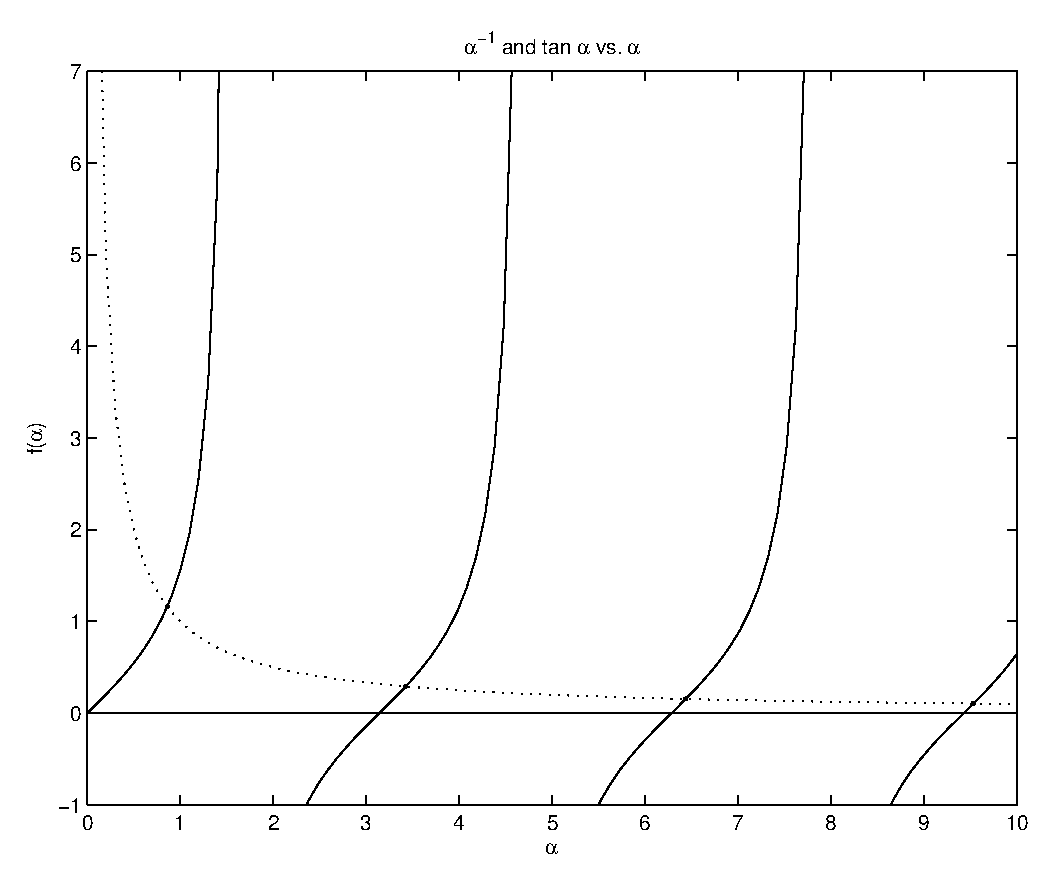
\includegraphics[width=250pt]{ModeRoots.eps}}
%\centerline{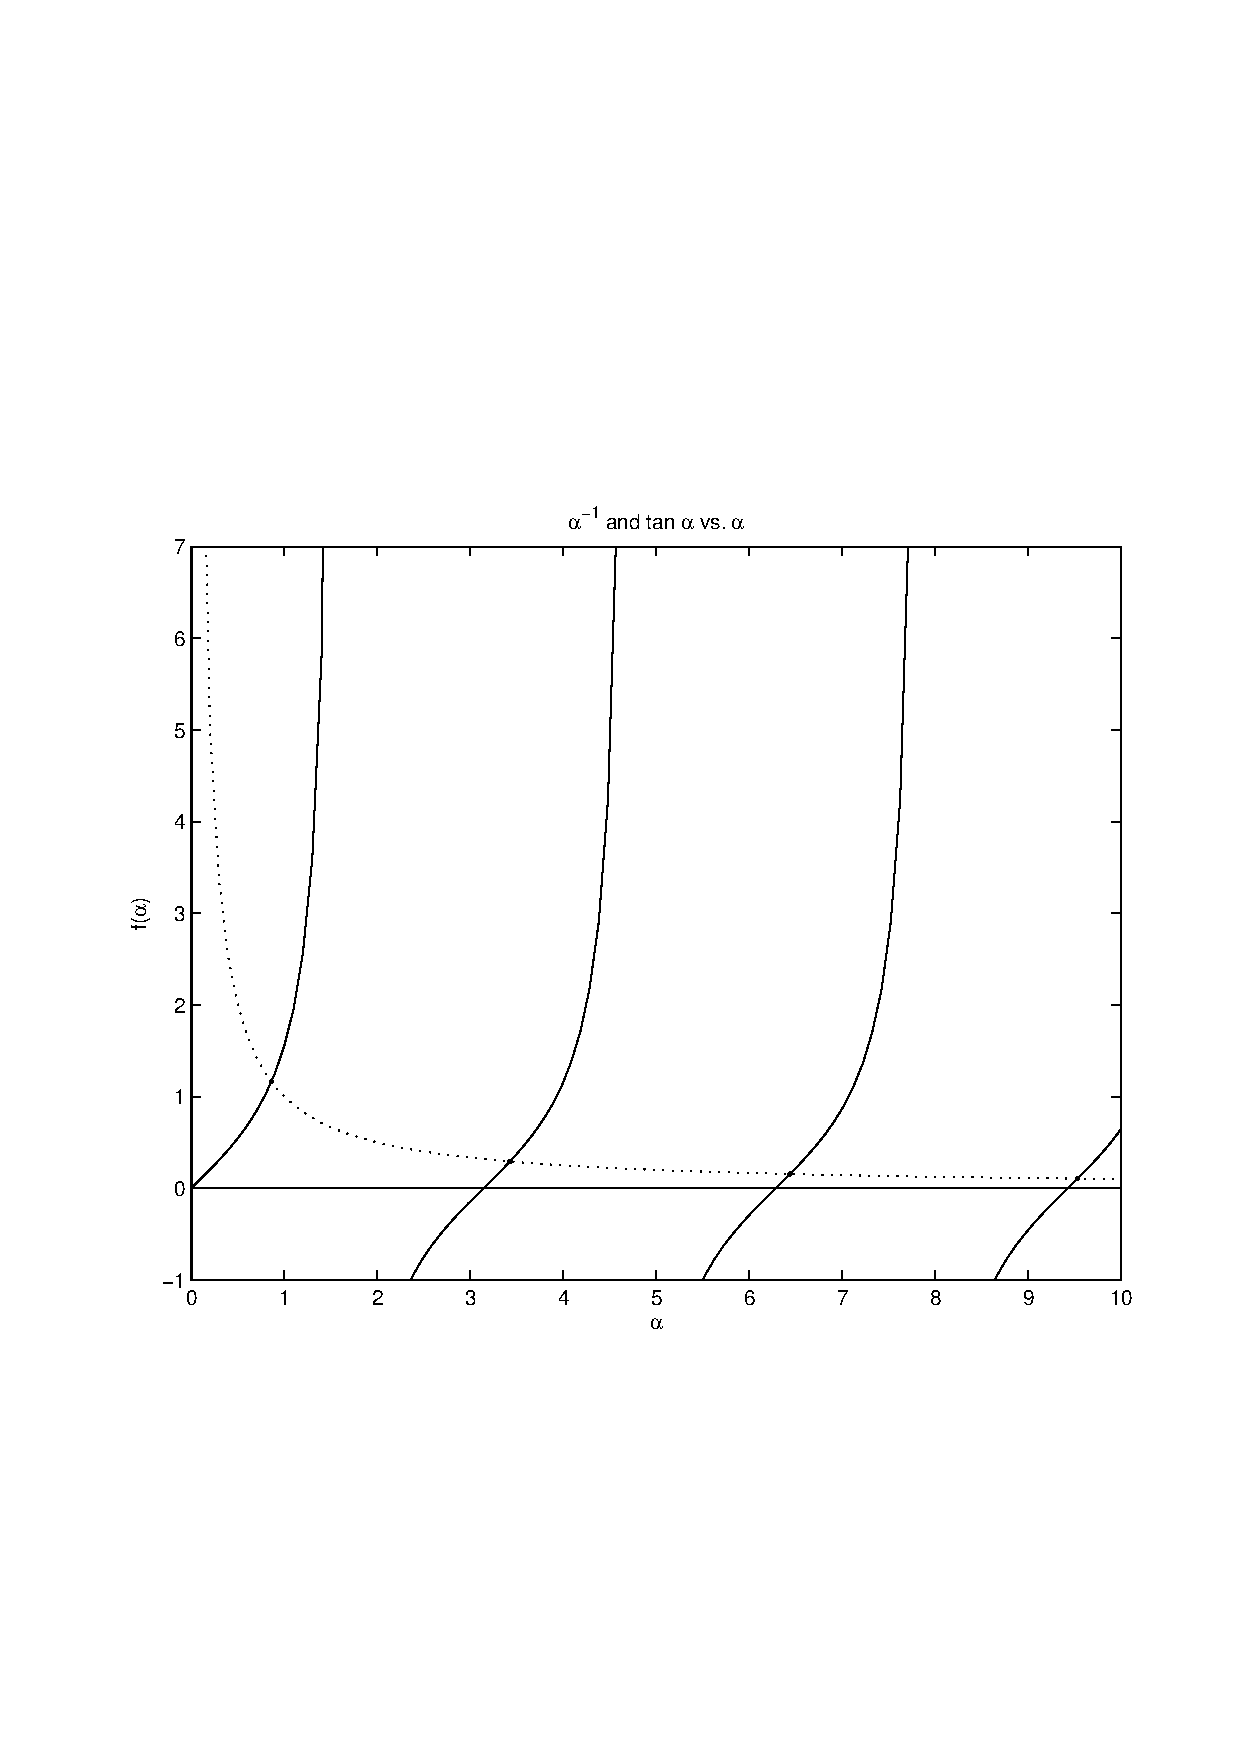
\includegraphics[width=250pt]{ModeRoots.png}}   %---For pdflatex
\caption{\footnotesize The solid line is the curve for $\tan \alpha$ and the dotted line is for $\alpha^{-1}$. The intersection of the curves correspond to the roots of the equation $\alpha^{-1} = \tan \alpha$. As $\alpha$ increases, we see that the roots approach $\alpha = \pi n$.}
\label{ModeRootsFig}
\end{figure}

We must now apply the boundary conditions to obtain a complete solution. From the surface condition, $G(z) = 0$ at $z = -D_*$, we see that
\begin{equation}
G(z) \simeq \frac{1}{\sqrt{N(z)}} \sin \left[\frac{1}{\sqrt{g D_n}} \int_{-D_*}^{z} N(z') dz' \right].
\end{equation}
From the upper condition, $G_z - G / D_n = 0$ at $z = 0$, and using the fact that $dN/dz$ is small, we find that
\begin{equation}
N \sqrt{\frac{D_n}{g}} = \tan \left[\frac{1}{\sqrt{g D_n}} \int_{-D_*}^{0} N(z') dz' \right].
\end{equation}
If we let $\alpha_n = \sqrt{\frac{g}{N^2 D_n}}$, then solving for $D_n$ is equivalent to solving for $\alpha_n$ in the equation
\begin{equation}\label{ModeRoots}
\frac{1}{\alpha_n} = \tan \left(k \alpha_n \right),
\end{equation}
where $k = \frac{N}{g} \int_{-D_*}^{0} N(z') dz'$. The solutions to this equation for $k=1$ are illustrated in figure \ref{ModeRootsFig}.
We can see that the roots correspond to $\alpha_n = \pi n / k$ as $n$ becomes large so that
\begin{equation}
D_n \simeq \frac{\left[\int_{-D_*}^{0} N(z') dz' \right]^2}{g \pi^2 n^2}.
\end{equation}
Although this is only formally correct for large $n$, the error is often no more than $10\%$ for $n=1$, and the accuracy only improves with increasing $n$, so that the WKB solution can usually be safely applied to the entire baroclinic spectrum.

%%%%%%%%%%%%%%%%%%%%%%%%%%%%%%%%%%%%%%%%%%%%%%%%%%%%%%%%%%%%%%%%%%%%%%%%%%%%%%%

\section{Laplace Tidal Equations}

From the above equations and the modal solution with respect to the $z$ axis we can derive the Laplace tidal equations,

\begin{subequations}
\begin{align*}
U_t - f V &= -\frac{g \zeta_\phi}{a \cos\theta}, \\
V_t + f U &= -\frac{g \zeta_\theta}{a},
\end{align*}
\begin{equation*}
\frac{U_\phi}{a\cos\theta}+\frac{(V\cos\theta)_\theta}{a\cos\theta}+\frac{W}{h_j} = 0,
\end{equation*}
\begin{equation*}
\zeta_t = W.
\end{equation*}
\end{subequations}

And if the two last equations are combined,

\begin{subequations}
\begin{align*}
U_t - f V &= -\frac{g \zeta_\phi}{a \cos\theta}, \\
V_t + f U &= -\frac{g \zeta_\theta}{a},
\end{align*}
\begin{equation*}
\zeta_t+h_j\left(\frac{U_\phi}{a\cos\theta}+\frac{(V\cos\theta)_\theta}{a\cos\theta}\right) = 0.
\end{equation*}
\end{subequations}

This set of equations for each mode was considered for a flat bottom and with no external forcing. The friction and the tidal gravitational potential (TGP) can be introduced by simply decomposing these functions into their vertical modes. But since the TGP does not vary significantly across the shallow depth of the fluid, only the barotropic mode is excited noticeably when the bottom is flat, despite the fact that actual observations show strong baroclinic tides.

Although we will not discuss how to approach the full baroclinic case, we can consider the barotropic mode over a variable topography with a weakly elastic bottom (due to the elasticity of the earth). In this case, let $D(\theta, \phi)$ describe the mean depth of a homogeneous fluid, and $\delta$ denote the displacement of the elastic bottom. Then the equations for the barotropic mode are generalized to
\begin{subequations}
\begin{align}
u_t - \left(2\Omega \sin \theta \right) v &= - \frac{g\left(\zeta - \Gamma/g \right)_\phi}{a \cos \theta} + \frac{F^{\phi}}{\rho D}, \\
v_t + \left(2\Omega \sin \theta \right) u &= - \frac{g\left(\zeta - \Gamma/g \right)_\theta}{a} + \frac{F^{\theta}}{\rho D},
\end{align}
\begin{equation}
\left(\zeta_t - \delta_t\right) + \frac{1}{a \cos \theta} \left[\left(u D \right)_\phi + \left(v D \cos \theta \right) \right] = 0.
\end{equation}
\end{subequations}
We will refer to these as the LTE. Note that an equation for the dynamics of the elastic bottom must be included to fully describe the system.

\vspace{5mm}
\noindent
\emph{Notes by Yaron Toledo and Marshall Ward.}

%...Can you get these equations out of the vertical mode decomposition??

%...Also, there is a potential notation problem here. Make sure it matches up with the next group's notation.

%%%%%%%%%%%%%%%%%%%%%%%%%%%%%%%%%%%%%%%%%%%%%%%%%%%%%%%%%%%%%%%%%%%%%%%%%%%%%%%

%\section{Conclusion}
%\label{conclusion}

% You can add your own bibliography file (say, mybib.bib) here:
\bibliography{gfd2004,lecture02}
%\bibliography{gfd2004}

\end{document}
